\documentclass[10 pt,usenames,dvipsnames, oneside]{article}
\usepackage{../../../modelo-ensino-medio}



\begin{document}

\begin{center}
  \begin{minipage}[l]{3cm}

\includegraphics[width=2cm]{logo}    
\end{minipage}\hfill
\begin{minipage}[r]{.8\textwidth}
 {\Large \scshape Atividade: Batalha Naval}  
\end{minipage}
\end{center}
\vspace{.2cm}

\ifdefined\prof
%Habilidades da BNCC
% \begin{objetivos}
% \item 
% \end{objetivos}

%Caixa do Para o Professor
\begin{goals}
%Objetivos específicos
\begin{enumerate}
\item Problematizar as curvas no plano como relações entre as variáveis $x$ e $y$.
\end{enumerate}

\tcblower

%Orientações e sugestões
\begin{itemize}
\item  O professor pode propor equações do tipo $ax+0y=c$ ou $0x+by=c$, para fazer o aluno perceber que é possível deixar uma das incógnitas livre. Isso ajudará o aluno a entender a resposta do item $e)$. Um aluno mais atento pode tentar importar as ideias das funções do segundo grau para descrever equações do segundo grau. Esse tipo de pensamento pode e deve ser trabalhado, de forma que se possa responder a questão $e)$. Outras possibilidades são as equações equivalentes $x = x, x-y = x-y,$ etc.
%
\item Nessa atividade, a prioridade é a investigação em detrimento da obtenção de uma resposta única. Usando o GeoGebra é possível investigar essa situação. Podemos, por exemplo, usar o comando POLINOMIO(<lista de pontos.) na cartela de Laís, e digitar os pontos A, B, C e verificando o que visualizamos na tela. Por exemplo, quando usamos POLINOMIO(A,B,C), visualizamos um polinômio do 2º grau na janela da álgebra mas, quando agregamos a esta lista de pontos, o ponto D, com o comando POLINOMIO(A,B,C,D) a curva desaparece da tela. Vale a pena problematizar essa questão com os alunos, considerando que como o comando POLINOMIO esboça gráficos de funções polinomiais cujos gráficos passam por um determinado conjunto de pontos, então o fato de que $A$ e $D$ estão alinhados inviabiliza que esse comando retorne um resultado gráfico ou algébrico. Da mesma forma ocorre com os pontos E e , também alinhados, e ainda com J, F e I.

O comando CURVAIMPLÍCITA(<listadepontos>) é usado da mesma forma que o comando POLINOMIO mas, em lugar de buscar uma função polinomial que contenha todos os pontos listados, ele busca uma curva e exibe sua equação. Com o comando curva implicita(A,B,C,D,E,F,G,H,I), conseguimos na cartela de Laís a curva.
\item Após a realização guiada dessa atividade, pode ser proposto que os alunos desenvolvam seus próprios tabuleiros e joguem entre si formando duplas e fazendo o papel de Laís e André
\end{itemize}
\end{goals}

\bigskip
\begin{center}
{\large \scshape Atividade}
\end{center}
\fi

Laís e André estão jogando uma batalha naval diferente: nesse jogo, cada jogador tem uma cartela, em formato de plano cartesiano, de maneira que os valores das incógnitas $x$ e $y$ pertençam ao intervalo $[-5,5]$. Cada jogador marca $10$ pontos em sua cartela, sempre com coordenadas inteiras. Os "tiros"{} são dados a partir de equações nas incógnitas $x$ e $y$ que devem "acertar"{} os pontos que tenham sido marcados na cartela do adversário. A equação "acerta"{} um ponto quando ele é solução da equação. Por exemplo: a equação $x+4y=5$ acerta o ponto $(4,1)$, pois $x = 4$ e $y = 1$ é solução da equação. Se a "equação-tiro"{} acertar mais de um ponto, então o jogador que acertou terá a pontuação igual ao quadrado do número de pontos que acertou.

Laís e André irão disputar uma partida do jogo e cada um já marcou os seus pontos nas cartelas. Veja como eles ficaram dispostos:

\begin{figure}[H]
\centering

\noindent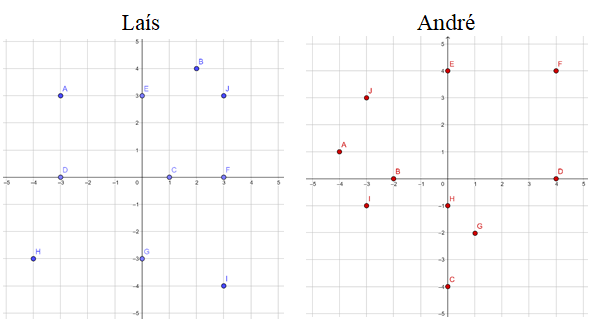
\includegraphics[width=375bp]{batalha.png}
\end{figure}

\begin{enumerate}
\item {}
	Laís é a primeira a jogar. Cite dois exemplos de equações-tiro que Laís pode dar para acertar pelo menos dois pontos marcados por André.

\item {}
	André, em sua jogada, usou $x^2 + y^2 = 9$ como equação-tiro. Qual a sua pontuação com essa jogada?

\item {}
	Dê exemplo de três equações-tiro que permitam à Laís acertar o ponto $A$ da cartela de André.

\item {}
	Suponha que Laís e André irão começar uma nova partida e que Laís inicie o jogo com a equação-tiro $x+2y = 4$. Dependendo dos pontos marcados por André em sua cartela, qual é a pontuação máxima que ela pode adquirir com essa jogada? Nesse caso, marque no plano cartesiano os pontos que ela terá acertado.

\item {}
	Com as regras que foram estabelecidas, existe alguma equação-tiro que André dê que acerte todos os pontos da cartela de Laís em uma única rodada?

\end{enumerate}

\ifdefined\prof
\begin{solucao}
\begin{enumerate}
\item $x+0y=0, 0x+y=0, x+0y=4, y+0x=4, 0x+y=-1, 4y-5x=-4; 2x-y=4; y+x=4,$ entre outras;
\item A equação de André passa por 4 pontos da cartela de Laís,  pontuando assim 16 pontos;
\item $2y+x=-2; y=2x+9; 4y-3x=16$;
\item A pontuação máxima é $25$, atingindo $5$ pontos, a saber 

$(-4,4); (-2,3); (0,2); (2,1); (4,0)$;
\item $0x+0y=0$.
\end{enumerate}
\end{solucao}
\fi

\end{document}